%!TEX program = xelatex
\documentclass[11pt]{beamer}

\usepackage{amsfonts}
\usepackage{amsmath}
\usepackage{blindtext}
\usepackage{enumitem}

\usetheme{SaoPaulo}

\title{Python Basics!}
\subtitle{mutability, container methods}
\author{CS101 Lecture \#9}
\date{2016-09-21}

\setcounter{showSlideNumbers}{1}

\begin{document}
  \setcounter{showProgressBar}{0}
  \setcounter{showSlideNumbers}{0}

%%%%%%%%%%%%%%%%%%%%%%%%%%%%%%%%%%%%%%%%%%%%%%%%%%%%%%%%%%%%%%%%%%%%%%%%%%%%%%%%
\frame{\titlepage}

%%%%%%%%%%%%%%%%%%%%%%%%%%%%%%%%%%%%%%%%%%%%%%%%%%%%%%%%%%%%%%%%%%%%%%%%%%%%%%%%
\setcounter{framenumber}{0}
\setcounter{showProgressBar}{1}
\setcounter{showSlideNumbers}{1}

%%%%%%%%%%%%%%%%%%%%%%%%%%%%%%%%%%%%%%%%%%%%%%%%%%%%%%%%%%%%%%%%%%%%%%%%%%%%%%%%
\section{Administrivia}

%%%%%%%%%%%%%%%%%%%%%%%%%%%%%%%%%%%%%%%%%%%%%%%%%%%%%%%%%%%%%%%%%%%%%%%%%%%%%%%%
\begin{frame}
  \frametitle{Administrivia}
  \Enlarge
  \begin{itemize}
  \myitem  Homework \#4 is due Friday Sep.\ 23.
  \myitem  Midterm \#1 will be Monday Oct.\ 3.  (evening)
  \end{itemize}
\end{frame}

%%%%%%%%%%%%%%%%%%%%%%%%%%%%%%%%%%%%%%%%%%%%%%%%%%%%%%%%%%%%%%%%%%%%%%%%%%%%%%%%
\section{Warmup Quiz}

%%%%%%%%%%%%%%%%%%%%%%%%%%%%%%%%%%%%%%%%%%%%%%%%%%%%%%%%%%%%%%%%%%%%%%%%%%%%%%%%
\begin{frame}[fragile]
  \frametitle{Question \#1}
  \Enlarge

  \begin{semiverbatim}
a = 1
def fun(a,b):
    return a + b
a = fun( a,a ) + a
  \end{semiverbatim}
  What is the final value of \texttt{a}?
  \begin{enumerate}[label=\Alph*]
  \item  \texttt{2}
  \item  \texttt{3}
  \item  \texttt{4}
  \end{enumerate}
\end{frame}

%%%%%%%%%%%%%%%%%%%%%%%%%%%%%%%%%%%%%%%%%%%%%%%%%%%%%%%%%%%%%%%%%%%%%%%%%%%%%%%%
\begin{frame}[fragile]
  \frametitle{Question \#1 (Worked)}
  \Enlarge

  \begin{semiverbatim}
a = 1
def fun(c,b):
    return c + b
a = fun( a,a ) + a
  \end{semiverbatim}
\end{frame}

%%%%%%%%%%%%%%%%%%%%%%%%%%%%%%%%%%%%%%%%%%%%%%%%%%%%%%%%%%%%%%%%%%%%%%%%%%%%%%%%
\section{Mutability \& Aliasing}

%%%%%%%%%%%%%%%%%%%%%%%%%%%%%%%%%%%%%%%%%%%%%%%%%%%%%%%%%%%%%%%%%%%%%%%%%%%%%%%%
\begin{frame}[fragile]
  \frametitle{Mutability}
  \Enlarge

  \begin{itemize}
  \myitem  We distinguished \emph{mutability} and \emph{immutability}.
  \myitem  The distinction arises from the storage in memory.
  \end{itemize}
  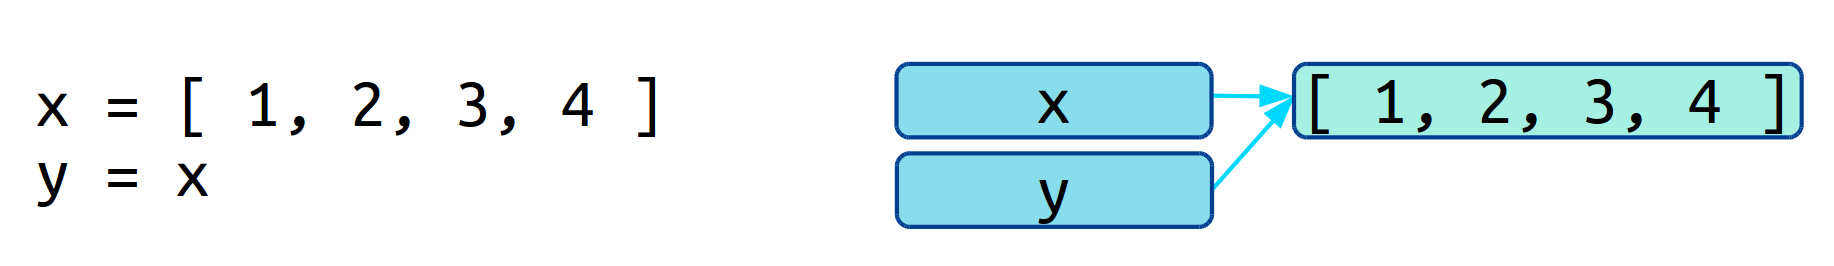
\includegraphics[width=0.8\textwidth]{./img/memory-mutability.png}
\end{frame}

%%%%%%%%%%%%%%%%%%%%%%%%%%%%%%%%%%%%%%%%%%%%%%%%%%%%%%%%%%%%%%%%%%%%%%%%%%%%%%%%
\begin{frame}[fragile]
  \frametitle{Mutability}
  \Enlarge

  \begin{itemize}
  \myitem  \emph{Immutability} occurs when values are copies in memory.
  \end{itemize}
  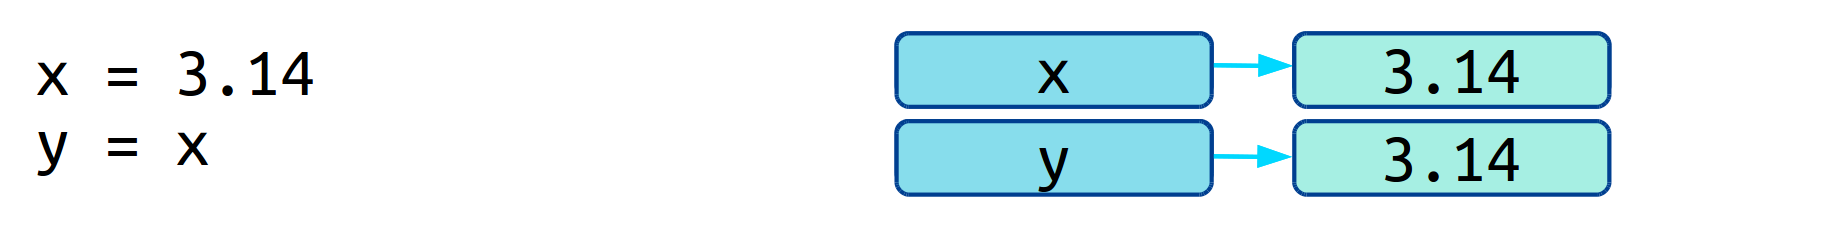
\includegraphics[\textwidth]{./img/memory-immutability.png} \\
  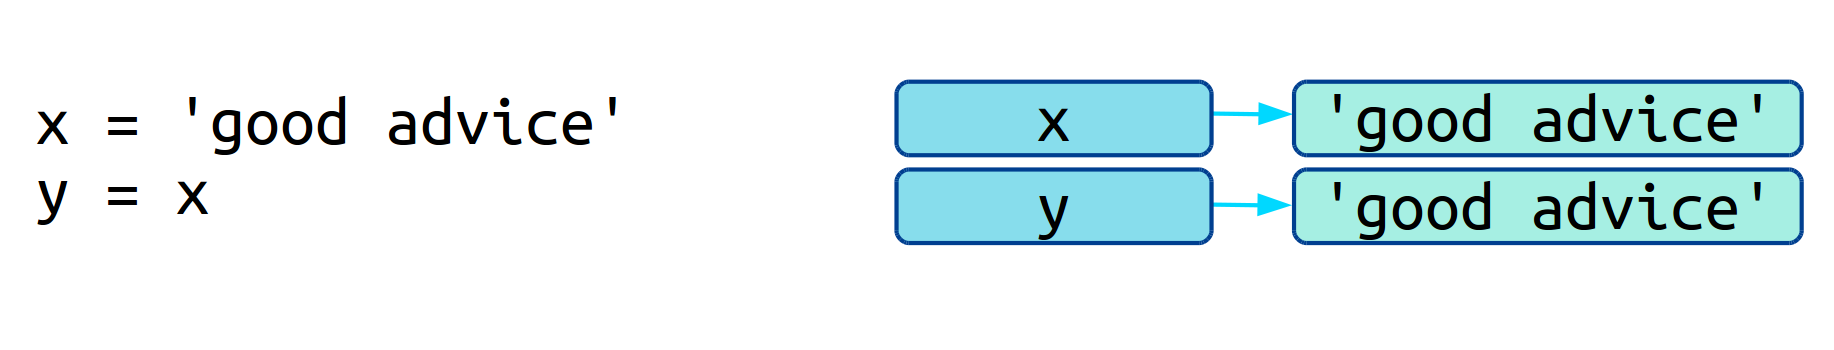
\includegraphics[\textwidth]{./img/memory-immutability-string.png}
\end{frame}

%%%%%%%%%%%%%%%%%%%%%%%%%%%%%%%%%%%%%%%%%%%%%%%%%%%%%%%%%%%%%%%%%%%%%%%%%%%%%%%%
\begin{frame}[fragile]
  \frametitle{Mutability \& immutability}
  \Enlarge

  \begin{itemize}
  \myitem  \emph{Mutability} occurs when values share the same location.
  \myitem  The distinction arises from the storage in memory.
  \end{itemize}
  \begin{semiverbatim}

  \end{semiverbatim}
\end{frame}

%%%%%%%%%%%%%%%%%%%%%%%%%%%%%%%%%%%%%%%%%%%%%%%%%%%%%%%%%%%%%%%%%%%%%%%%%%%%%%%%
\begin{frame}[fragile]
  \frametitle{Aliasing}
  \Enlarge

  \begin{itemize}
  \myitem  \emph{Aliasing} occurs when one memory location has two names.
  \myitem  \textcolor{red}{Aliasing causes mutable types to behave unexpectedly!}
  \end{itemize}
  \begin{semiverbatim}

  \end{semiverbatim}
\end{frame}

%%%%%%%%%%%%%%%%%%%%%%%%%%%%%%%%%%%%%%%%%%%%%%%%%%%%%%%%%%%%%%%%%%%%%%%%%%%%%%%%
\begin{frame}[fragile]
  \frametitle{Aliasing}
  \Enlarge

  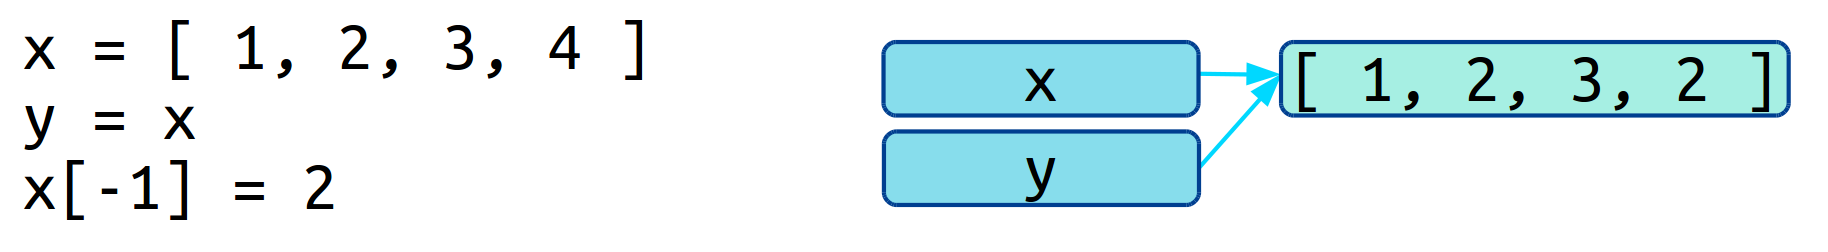
\includegraphics[0.8\textwidth]{./img/memory-aliasing.png}
\end{frame}

%%%%%%%%%%%%%%%%%%%%%%%%%%%%%%%%%%%%%%%%%%%%%%%%%%%%%%%%%%%%%%%%%%%%%%%%%%%%%%%%
\begin{frame}[fragile]
  \frametitle{Example}
  \Enlarge

  \begin{semiverbatim}
a = [ 'a', 'b', 'c', 'd' ]
b = a
b[3] = '*'
  \end{semiverbatim}
  What is the final value of \texttt{a}?
  \begin{enumerate}[label=\Alph*]
  \item  \texttt{[ 'a', 'b', '*', 'd' ]}
  \item  \texttt{[ 'a', 'b', 'c', '*' ]}
  \item  \texttt{[ 'a', 'b', 'c', 'd' ]}
  \item  None of the above.
  \end{enumerate}
\end{frame}

%%%%%%%%%%%%%%%%%%%%%%%%%%%%%%%%%%%%%%%%%%%%%%%%%%%%%%%%%%%%%%%%%%%%%%%%%%%%%%%%
\begin{frame}[fragile]
  \frametitle{Tuples}
  \Enlarge

  \begin{itemize}
  \myitem  The immutable analogue of a \texttt{list} is a \texttt{tuple}.
  \myitem  We form a tuple by using parentheses \texttt{()} instead of square brackets \texttt{[]}.
  \end{itemize}
\end{frame}

%%%%%%%%%%%%%%%%%%%%%%%%%%%%%%%%%%%%%%%%%%%%%%%%%%%%%%%%%%%%%%%%%%%%%%%%%%%%%%%%
\section{Container Methods}

%%%%%%%%%%%%%%%%%%%%%%%%%%%%%%%%%%%%%%%%%%%%%%%%%%%%%%%%%%%%%%%%%%%%%%%%%%%%%%%%
\begin{frame}[fragile]
  \frametitle{Container Methods}
  \Enlarge

  \begin{itemize}
  \myitem  Because \texttt{list}s are mutable, we can change their contents.
  \end{itemize}
  \begin{semiverbatim}
x = [ 4,1,2,3 ]
x[3] = -2       # item assignment
x.append(5)     # appending items
del x[1]        # removing items
x.sort()        # changing item order
  \end{semiverbatim}
\end{frame}

%%%%%%%%%%%%%%%%%%%%%%%%%%%%%%%%%%%%%%%%%%%%%%%%%%%%%%%%%%%%%%%%%%%%%%%%%%%%%%%%
\begin{frame}[fragile]
  \frametitle{Container Methods}
  \Enlarge

  \begin{itemize}
  \myitem  \texttt{sort} and \texttt{append} modify the \texttt{list} itself.
  \end{itemize}
  \begin{alertblock}{Warning!}
  This means that \texttt{sort} and \texttt{append} \texttt{return None}!
  \end{alertblock}
  \begin{semiverbatim}
x = [ 4,1,2,3 ]
x.sort()        # This is the right way to sort a list.
print(x)
  \end{semiverbatim}
\end{frame}

%%%%%%%%%%%%%%%%%%%%%%%%%%%%%%%%%%%%%%%%%%%%%%%%%%%%%%%%%%%%%%%%%%%%%%%%%%%%%%%%
\begin{frame}[fragile]
  \frametitle{Container Methods}
  \Enlarge

  \begin{itemize}
  \myitem  \texttt{sort}, \texttt{reverse}, and \texttt{append} modify the \texttt{list} itself.
  \end{itemize}
  \begin{alertblock}{Warning!}
  This means that \texttt{sort} and \texttt{append} \texttt{return None}!
  \end{alertblock}
  \begin{semiverbatim}
x = [ 4,1,2,3 ]
x = x.sort()    # MANY of you will do this.  This is wrong!
print(x)
  \end{semiverbatim}
\end{frame}

%%%%%%%%%%%%%%%%%%%%%%%%%%%%%%%%%%%%%%%%%%%%%%%%%%%%%%%%%%%%%%%%%%%%%%%%%%%%%%%%
\begin{frame}[fragile]
  \frametitle{Example}
  \Enlarge

  \begin{semiverbatim}
y = [ 3,2,1 ]
x = y.append( 5 )
y[-1] = 3
  \end{semiverbatim}
  What is the final value of \texttt{x}?
  \begin{enumerate}[label=\Alph*]
  \item  \texttt{[ 3, 2, 1, 3 ]}
  \item  \texttt{[ 3, 2, 1, 5 ]}
  \item  \texttt{[ 3, 2, 1 ]}
  \item  \texttt{None}
  \end{enumerate}
\end{frame}

%%%%%%%%%%%%%%%%%%%%%%%%%%%%%%%%%%%%%%%%%%%%%%%%%%%%%%%%%%%%%%%%%%%%%%%%%%%%%%%%
\begin{frame}[fragile]
  \frametitle{Container Methods}
  \Enlarge

  \begin{itemize}
  \myitem  \texttt{index} returns the index of the first occurrence of a value in a \texttt{list}.
  \myitem  \texttt{count} returns how many times a value occurs.
  \myitem  \texttt{in} returns membership in the \texttt{list}.
  \myitem  \texttt{max}, \texttt{min}, \texttt{len}, etc.
  \end{itemize}
\end{frame}

%%%%%%%%%%%%%%%%%%%%%%%%%%%%%%%%%%%%%%%%%%%%%%%%%%%%%%%%%%%%%%%%%%%%%%%%%%%%%%%%
\section{Reminders}

%%%%%%%%%%%%%%%%%%%%%%%%%%%%%%%%%%%%%%%%%%%%%%%%%%%%%%%%%%%%%%%%%%%%%%%%%%%%%%%%
\begin{frame}
  \frametitle{Reminders}
  \Enlarge

  \begin{itemize}
  \myitem  Homework \#4 is due Friday Sep.\ 23.
  \myitem  Midterm \#1 will be Monday Oct.\ 3.  (evening)
  \end{itemize}
\end{frame}

\end{document}
